\documentclass{standalone}
\usepackage{tikz}
\usepackage{pgfplots}
\pgfplotsset{compat=1.18}

\begin{document}
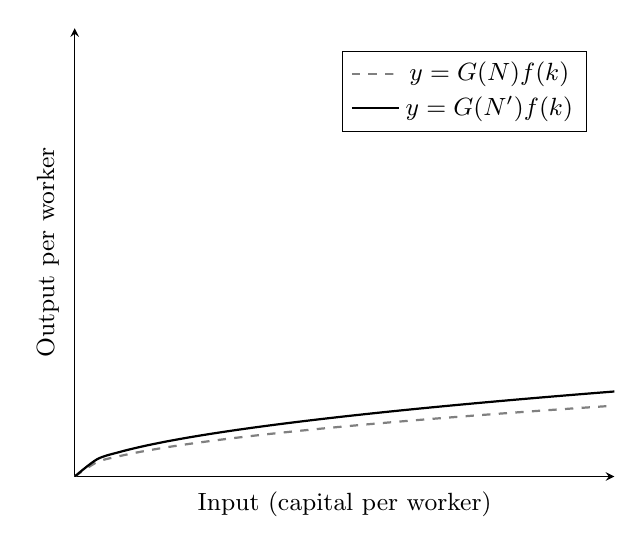
\begin{tikzpicture}
    \begin{axis}[
        xlabel={Input (capital per worker)},
        ylabel={Output per worker},
        xmin=0, xmax=10,
        ymin=0, ymax=10,
        axis lines=left,
        enlargelimits=false,
        xtick=\empty,
        ytick=\empty,
        label style={font=\small},
        legend style={at={(0.95,0.95)}, anchor=north east, font=\small},
    ]
        % Curve for G(N)f(k)
        \addplot [domain=0:10, smooth, thick, gray, dashed] {0.5*x^(0.5)};
        \addlegendentry{$y=G(N)f(k)$}

        % Curve for G(N')f(k)
        \addplot [domain=0:10, smooth, thick, black] {0.6*x^(0.5)};
        \addlegendentry{$y=G(N')f(k)$}
    \end{axis}
\end{tikzpicture}
\end{document}